\documentclass[tikz, border=8pt]{standalone}
\usepackage{tikz}
\usepackage{amsmath}
\usepackage{xcolor}
\usetikzlibrary{positioning, arrows.meta, shapes.geometric, fit, backgrounds, calc, decorations.pathmorphing}

% Color palette (consistent with arxiv-style serif body) -- see AGENTS.md rule 1
\definecolor{cAudio}{HTML}{F2F4F7}
\definecolor{cEnc}{HTML}{D9E5F4}
\definecolor{cEncB}{HTML}{4A7BB7}
\definecolor{cAdp}{HTML}{D9F0DA}
\definecolor{cAdpB}{HTML}{4F9D58}
\definecolor{cLLM}{HTML}{FBE3CC}
\definecolor{cLLMB}{HTML}{D08A3F}
\definecolor{cText}{HTML}{F2F4F7}
\definecolor{cPrompt}{HTML}{F7F2E8}
\definecolor{cPromptB}{HTML}{B89464}
\definecolor{cTok}{HTML}{EEE8F4}
\definecolor{cTokB}{HTML}{6A4DA8}
\definecolor{cBound}{HTML}{F2DEDE}
\definecolor{cBoundB}{HTML}{B8585F}
\definecolor{cMerge}{HTML}{FFF7D6}
\definecolor{cMergeB}{HTML}{C5A53E}
\definecolor{cFrozen}{HTML}{8A8A8A}
\definecolor{cTrain}{HTML}{2F6FB1}
\definecolor{cTune}{HTML}{2F8E40}

\tikzset{
  module/.style    ={draw, rounded corners=3pt, minimum width=3.4cm, minimum height=1.05cm,
                     align=center, font=\sffamily\small, line width=0.7pt},
  audio/.style     ={module, fill=cAudio, draw=black!40},
  encoder/.style   ={module, fill=cEnc, draw=cEncB},
  adapter/.style   ={module, fill=cAdp, draw=cAdpB},
  llm/.style       ={module, fill=cLLM, draw=cLLMB, minimum width=8.4cm, minimum height=1.5cm},
  textout/.style   ={module, fill=cText, draw=black!40, minimum width=2.6cm},
  tokbox/.style    ={module, fill=cTok, draw=cTokB},
  boundbox/.style  ={module, fill=cBound, draw=cBoundB},
  mergebox/.style  ={module, fill=cMerge, draw=cMergeB, minimum width=8.4cm, minimum height=0.95cm,
                     font=\sffamily\small\itshape},
  flow/.style      ={-Stealth, line width=0.8pt, draw=black!70},
  rateflow/.style  ={-Stealth, line width=0.6pt, draw=black!55, dashed},
  ratelabel/.style ={font=\sffamily\scriptsize, text=black!55},
  tag/.style       ={font=\sffamily\tiny, inner sep=1pt}
}

\begin{document}
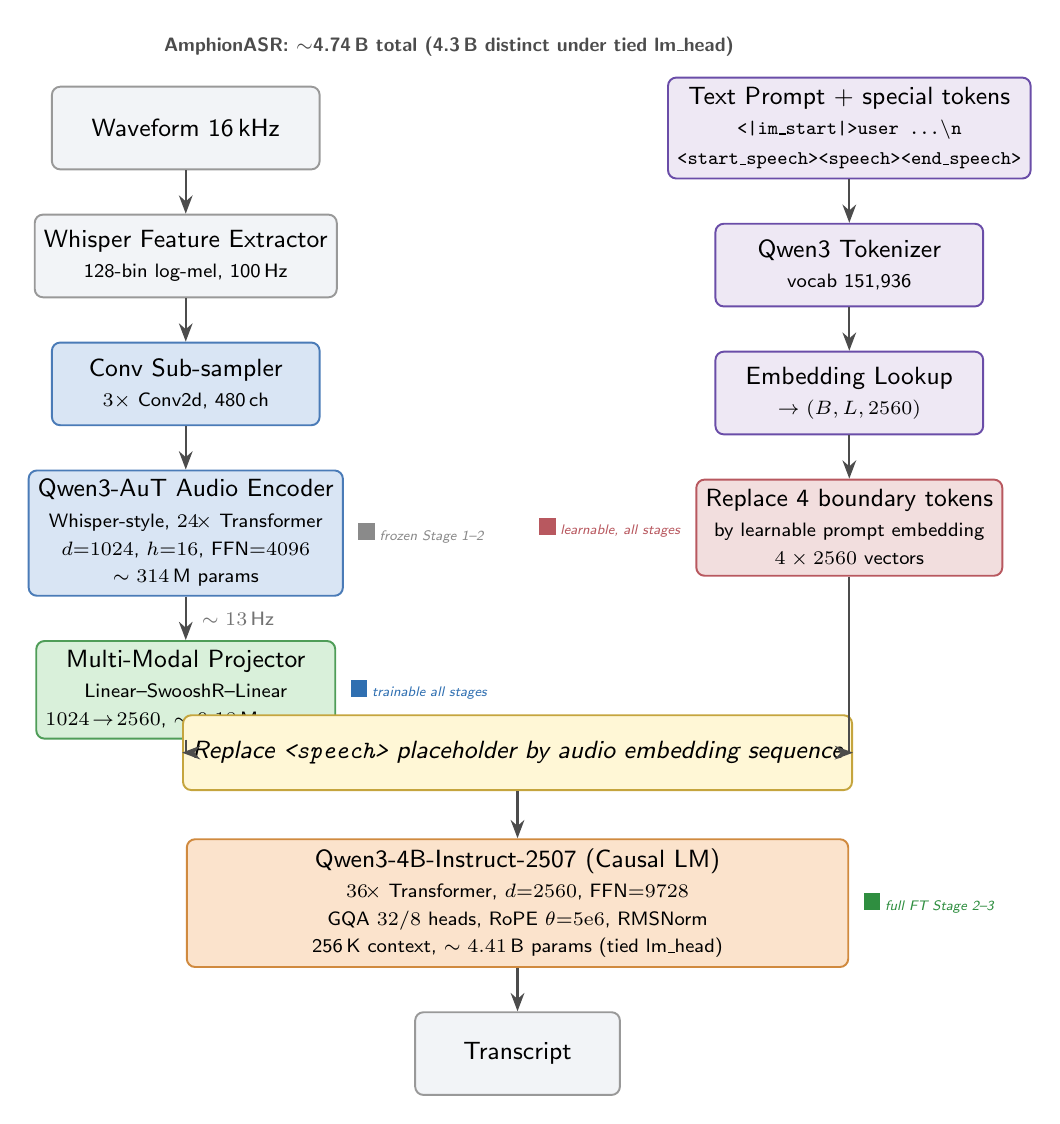
\begin{tikzpicture}[node distance=0.55cm and 0.6cm]

  % ====================== Audio branch (left column) ======================
  \node[audio]    (waveform) {Waveform 16\,kHz};
  \node[audio,    below=of waveform] (mel) {%
    Whisper Feature Extractor\\
    \scriptsize 128-bin log-mel, 100\,Hz
  };
  \node[encoder,  below=of mel] (conv) {%
    Conv Sub-sampler\\
    \scriptsize $3\times$ Conv2d, 480\,ch
  };
  \node[encoder,  below=of conv] (qwenaut) {%
    Qwen3-AuT Audio Encoder\\
    \scriptsize Whisper-style, $24\!\times$ Transformer\\[-1pt]
    \scriptsize $d{=}1024$, $h{=}16$, FFN${=}4096$\\[-1pt]
    \scriptsize $\sim314$\,M params
  };
  \node[adapter,  below=of qwenaut] (proj) {%
    Multi-Modal Projector\\
    \scriptsize Linear--SwooshR--Linear\\[-1pt]
    \scriptsize $1024 \!\to\! 2560$, $\sim9.18$\,M params
  };

  \draw[flow] (waveform) -- (mel);
  \draw[flow] (mel)      -- (conv);
  \draw[flow] (conv)     -- (qwenaut);
  \draw[flow] (qwenaut)  -- (proj)
        node[midway, right=2pt, ratelabel] {$\sim13$\,Hz};

  % ====================== Text branch (right column) ======================
  \node[tokbox, right=4.4cm of waveform] (prompt) {%
    Text Prompt + special tokens\\
    \scriptsize \texttt{<{}|{}im\_start{}|{}>user \dots\textbackslash n}\\
    \scriptsize \texttt{<start\_speech><speech><end\_speech>}
  };
  \node[tokbox, below=of prompt] (tok) {%
    Qwen3 Tokenizer\\
    \scriptsize vocab 151{,}936
  };
  \node[tokbox, below=of tok] (embed) {%
    Embedding Lookup\\
    \scriptsize $\to (B,L,2560)$
  };
  \node[boundbox, below=of embed] (bound) {%
    Replace 4 boundary tokens\\
    \scriptsize by learnable prompt embedding\\[-1pt]
    \scriptsize $4 \times 2560$ vectors
  };

  \draw[flow] (prompt) -- (tok);
  \draw[flow] (tok)    -- (embed);
  \draw[flow] (embed)  -- (bound);

  % ====================== Merge & LLM ======================
  \node[mergebox] at ($(proj.south) ! 0.5 ! (bound.south) + (0,-1.2)$) (merge)
        {Replace \texttt{<speech>} placeholder by audio embedding sequence};

  \draw[flow] (proj.south)  |- (merge.west);
  \draw[flow] (bound.south) |- (merge.east);

  \node[llm, below=0.6cm of merge] (llm) {%
    Qwen3-4B-Instruct-2507 (Causal LM)\\
    \scriptsize $36\!\times$ Transformer, $d{=}2560$, FFN${=}9728$\\[-1pt]
    \scriptsize GQA $32/8$ heads, RoPE $\theta{=}5\mathrm{e}6$, RMSNorm\\[-1pt]
    \scriptsize 256\,K context, $\sim4.41$\,B params (tied lm\_head)
  };

  \draw[flow] (merge) -- (llm);

  \node[textout, below=of llm] (text) {Transcript};
  \draw[flow] (llm) -- (text);

  % ====================== Trainability tags ======================
  \node[tag, right=4pt of qwenaut.east, text=cFrozen]
        {{\color{cFrozen}\rule{6pt}{6pt}}\ \emph{frozen Stage 1--2}};
  \node[tag, right=4pt of proj.east, text=cTrain]
        {{\color{cTrain}\rule{6pt}{6pt}}\ \emph{trainable all stages}};
  \node[tag, right=4pt of llm.east, text=cTune]
        {{\color{cTune}\rule{6pt}{6pt}}\ \emph{full FT Stage 2--3}};
  \node[tag, left=4pt of bound.west, text=cBoundB]
        {{\color{cBoundB}\rule{6pt}{6pt}}\ \emph{learnable, all stages}};

  % ====================== Title banner ======================
  \node[font=\sffamily\scriptsize\bfseries, above=0.25cm of waveform.north,
        text=black!70, anchor=south west, xshift=-0.4cm]
        {AmphionASR: $\sim$4.74\,B total (4.3\,B distinct under tied lm\_head)};

\end{tikzpicture}
\end{document}
